 \subsection{Modificación de elementos de un arreglo}
	\subsubsection{Saturación del canal de memoria}
		Con el objetivo de analizar el impacto de los accesos a memoria de multiples núcleos realizamos un experimento en el cual cada uno de los dos núcleos accede a una mitad del arreglo concurrentemente modificando los valores, realizando un incremento en uno del valor correspondiente.
		
	\begin{center}
 	    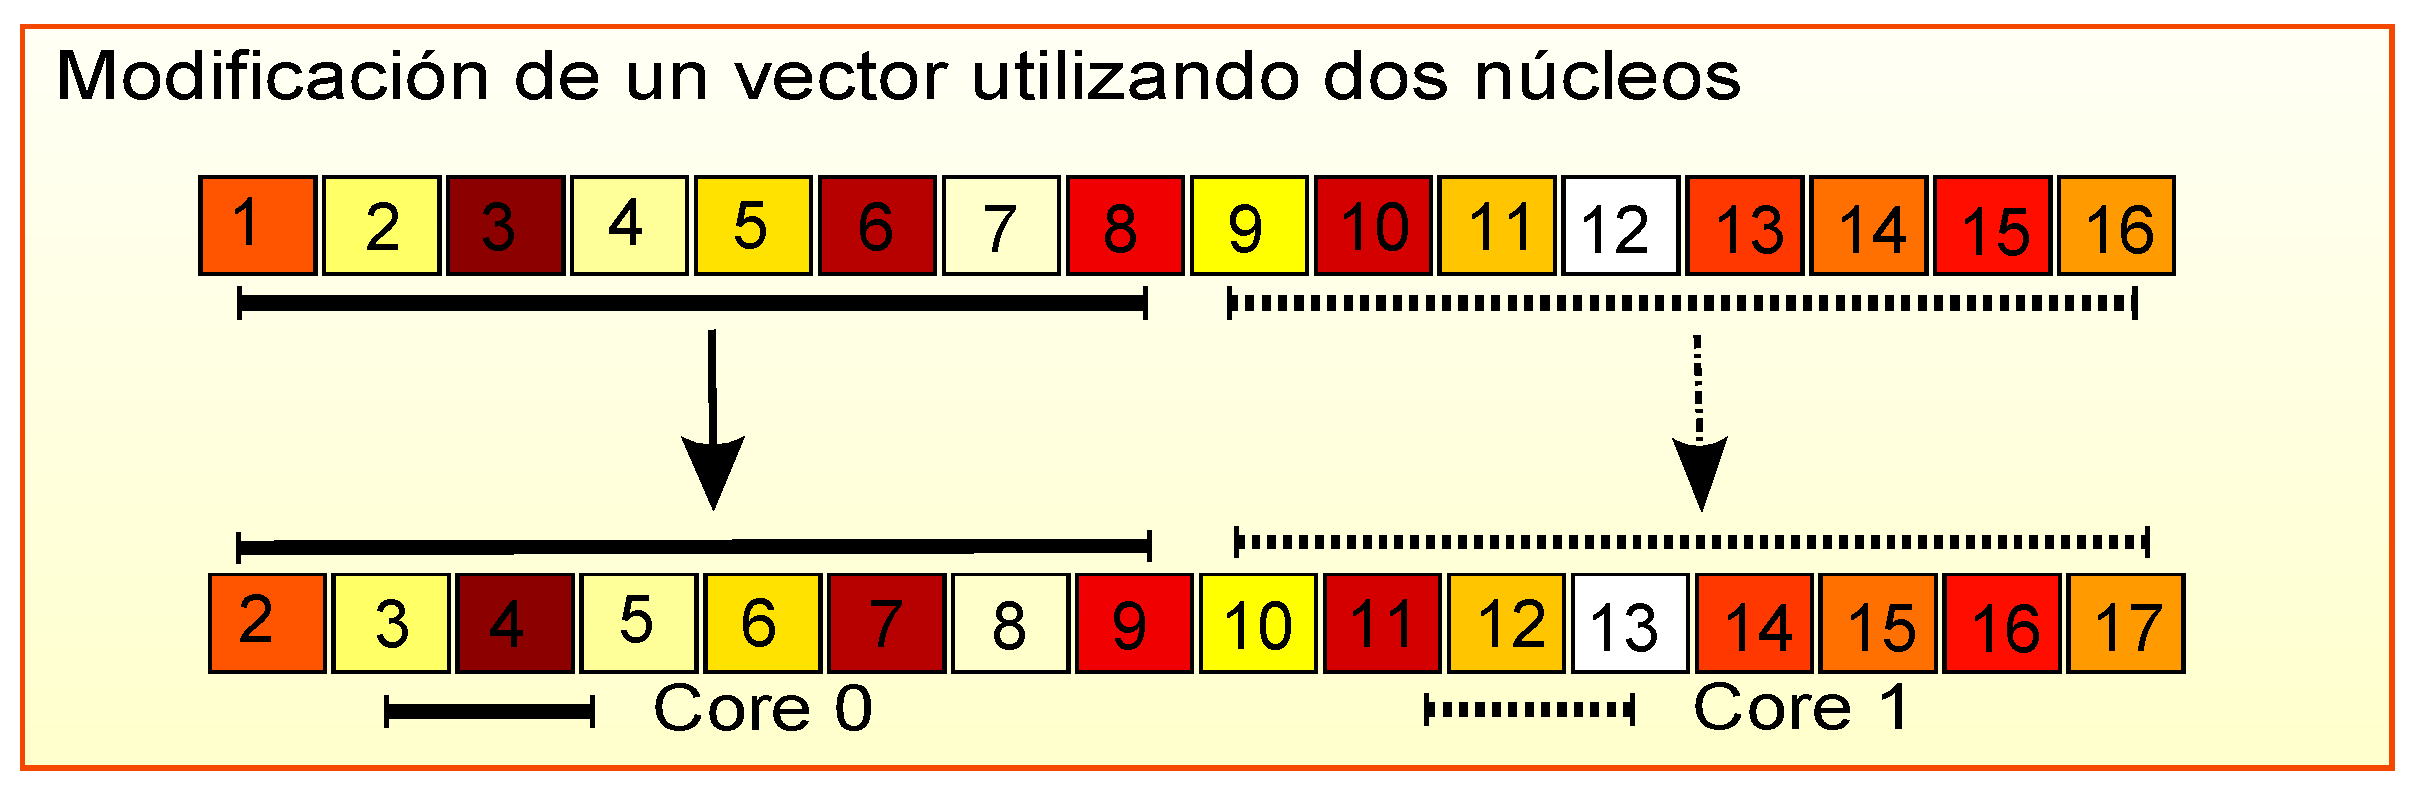
\includegraphics[height=4cm]{images/dualcore-vectorsum.pdf}
    \end{center}

	\subsubsection{Sincronizacion entre núcleos}
		En este algoritmo se realizo una sincronización sencilla de espera activa con roles master y slave, el protocolo es:
		\begin{enumerate}
			\item El master setea una bandera indicando al slave que comience su trabajo.
			\item El slave, que estaba realizando polling sobre la bandera del punto anterior comienza su trabajo, al finalizar, escribe en otra bandera indicando que finalizo.
			\item El master, luego de finalizar su trabajo, hace polling sobre una bandera en espera de la finalización del slave. Al salir de esta espera, concluye el algoritmo.
		\end{enumerate}
		
		\begin{center}
 	       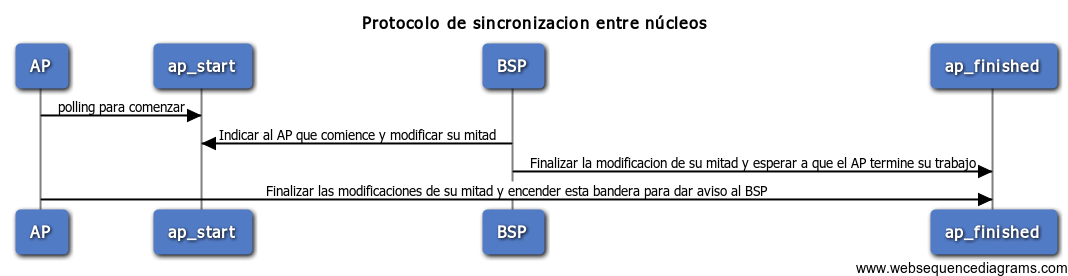
\includegraphics[height=4cm]{images/sync-vectorsum-seq.png}
    	\end{center}
